\chapter{Implementation of the mem-HNN hardware}

\section{Zielsetzung und Forschungsmethodik}
Upon establishing the precise research methodology, this chapter delves into the practical application of the previously mentioned methods.
First, the analysis phase of the \ac{DSR} process is executed with the goal to establish a model of the research plan 
which the requirements and framework conditions of the \ac{IT}-solution can be derived from. 
Next, the practical implementation is performed during the iterative design phase and uses the method of prototyping.
In the end of the design phase is a functional \ac{IT}-artifact, which fulfills the set requirements.
The evaluation phase in this chapter uses the method of simulation to answer the second part of the research question; to see how efficient 
the \ac{mem-HNN} can utilize the AI-model in terms of throughput and energy usage.

\section{Analysis phase}
\subsection{General conditions}
The first phase of the \ac{DSR}-cycle has the goal of specifying the objective and establishing an according research outline and the requirements of the artifact.
Additionally, the research outline should be visualized as a model of the overall solution concept.\footcite[cf.][278-279]{oesterleKonsortialforschung2010}
The objective of the practical part is already specified in chapter 3.1.
The underlying motivation hereby is to research if the known proof of concepts are feasible on the complete \ac{mem-HNN}
and evaluate if that brings an actual acceleration, which is equivalent to answering the research question of this thesis. 
This is tested by implementing the concept in software that is also part of the ASIC design process.\footnote{cf.\cite{raoUltimateGuideASIC}, p. 1; cf.\cite{ASICDesignFlow}, p. 1}

The implementaton is executed in the programming language Python since it offers a variety of third party libraries that are useful 
for machine learning that are state of the art, like pytorch, scikit learn etc..\footcite[cf.][306-307]{DiscreteContinuousModels}
Furthermore, sciki learn is chosen as machine learning library since it is the one of the industry standards for classical machine learning, has a broad variety of features in terms of \ac{RBM}s
and has a lower learning curve compared with e.g. Tensorflow.\footcite[cf.][5-6]{raschkaMachineLearningPython2020}

It should also be clarified that the analog \ac{mem-HNN}-accelerator consists of is implemented in software. 
This design decision is made out of time constraints of this thesis. 
Nonetheless, the complete hardware is is realizable in software without taking compromisses within their functionality.
The simulation data gathered later on is close to the actual energy efficiency and throughput. 



\begin{figure}[H]
    \centering
    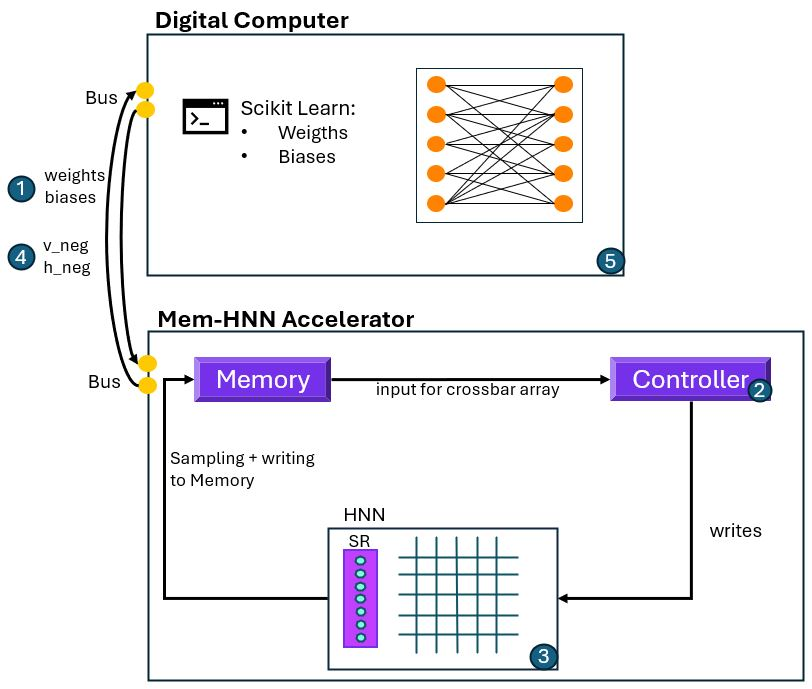
\includegraphics[width=0.80\linewidth]{graphics/Analysemodell.JPG}
    \caption{proposed solution architecture}
    \label{Overall architecture}
\end{figure}

\section{Design phase}



-Testen der Aktivierungsfunktion, wenn ich ein Neuron trainiere und dann Mitteln 
- Von vornerein auf Netzwerk Basis arbeiten mit mehren Neuron, jedoch für 1 Neuron testen



Hopfield Netzwerk aktivierungsfunktion der Updating methode

-> Konzeptionell Art des Updates mit keiner Temperatur wie bei MCMC 
Unterschied von MCMC zu Hopfield Netzwerk -> Zufällige Konfiguration und minimale Energie finden. Jedoch hat ein Hopfield
Netzwerk keine Temperatur 

-> Starte zufällige Konfiguration
-> Wähle ein Neuron aus und Berechne Summe und addiere mit Bias, 
-> Update wenn thresshold überschritten 1 und dann auf 0 
-> Speichern der neuen Konfuguration 
-> Starte iteration von gespeicherter Konfiguration 
-> Am Ende habe ich 10000 Vektoren (Die Konfigurationen) -> V1 Neuron wurde so und so oft aktiviert und ich muss average
über das neuron und habe dadurch die Aktivierungswarscheinlichkeit.

-Aktivierungsfunktion einfügen (Binary Step und verfleich zu sigmoid von Abb.4)



\section{Evaluation phase}

Aufbau der Simulator Pipeline
KI-Bibliothek Scikit-Learn
Evaluationsphase

To integrate simulation into the DSR concept ... 
The desired result of the prototyping is completing the \ac{DSR} design phase and with a simulation the result should be verified.
The input is the finished prototype, that mirrors the functionalities of the \ac{ASIC} on a high level.
